%% LaTeX Beamer presentation template (requires beamer package)
%% see http://latex-beamer.sourceforge.net/
%% idea contributed by H. Turgut Uyar
%% template based on a template by Till Tantau
%% this template is still evolving - it might differ in future releases!

\documentclass{beamer}

\usepackage{graphicx}
\usepackage{algorithmic}
\usepackage{algorithm}
\usepackage{listings}
\usepackage{booktabs}
\usepackage{amsmath}
\usepackage{setspace}
\usepackage{verbatim}
\usepackage{color}

\mode<presentation>
{
\usetheme{CambridgeUS}

\setbeamercovered{transparent}
}

\usepackage[english]{babel}
\usepackage[latin1]{inputenc}

% font definitions, try \usepackage{ae} instead of the following
% three lines if you don't like this look
\usepackage{mathptmx}
\usepackage[scaled=.90]{helvet}
\usepackage{courier}


\usepackage[T1]{fontenc}

\title{Compiler Design II}

\subtitle{\textsc{Design and Implementation of Recorder Analyzer}}

% - Use the \inst{?} command only if the authors have different
%   affiliation.
%\author{F.~Author\inst{1} \and S.~Another\inst{2}}
\author[Aronis \& Koukos]{Stavros Aronis \\ Konstantinos Koukos}

% - Use the \inst command only if there are several affiliations.
% - Keep it simple, no one is interested in your street address.
\institute[Uppsala University]
{
\textsc{\Large Uppsala University}\\[0.1cm]
\textsc{\Large Department of Information Technology}\\[2.0cm]
\vfill
}

\date{\today}

\begin{document}

\begin{frame}
\titlepage
\end{frame}

\begin{frame}
\frametitle{Outline}
\tableofcontents[hideallsubsections]
% You might wish to add the option [pausesections]
\end{frame}

\section{Motivation}

\subsection[Problem Presentation]{Problem Presentation}
\begin{frame}
  \frametitle{Problem Presentation}
  
  \begin{itemize}
  \item Erlang supports records with named fields
  \item Operations:
    \begin{itemize}
    \item Create new instance (possibly using default values)
    \item Retrieve a specific field
    \item Pattern match on multiple fields
    \item Create a new record from an existing one updating some fields
    \end{itemize}
  \item Records are often used to represent ``state''
  \end{itemize}
\end{frame}

\begin{frame}
  \frametitle{Problem Presentation}
  \begin{itemize}
  \item Records are implemented internally with tuples
  \item Erlang passes terms by reference...
    \pause
  \item ... except when it doesn't!
    \begin{itemize}
    \item Spawning a new process
    \item Sending a message to a process
    \item Storing a term in an Elang Term Storage table
    \item ... pretty printing a term to stdout!
    \end{itemize}
    \pause
  \item In these cases the term is copied to the heap of the destination
    process
  \item Copying large terms can take some time and can also result in terms of
    bigger size in the destination (in the current version, copying destroys
    sharing within a term)
  \end{itemize}
\end{frame}

\begin{frame}
  \frametitle{Problem Presentation}
  
  \begin{figure}
    \centering
    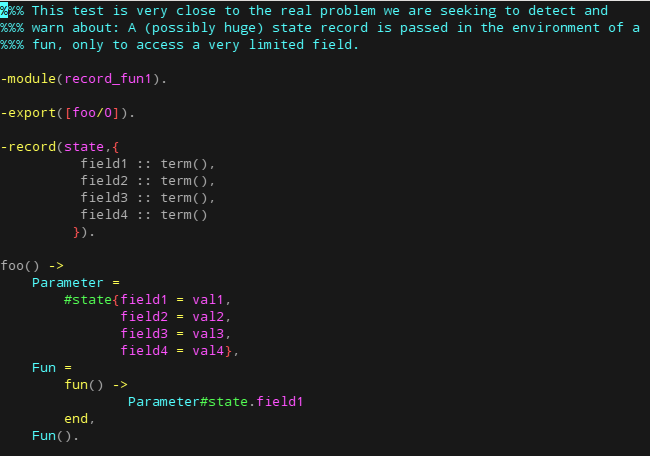
\includegraphics[scale=0.45]{../figures/problem_introduction}
  \end{figure}
  
\end{frame}

\begin{frame}
  \frametitle{Solution Introduction}
  
  \begin{itemize}
  \item The Recorder Analyzer:
    \begin{itemize}
    \item Detect cases where an argument is treated as a record but not all
      fields are accessed
    \item Automatic optimization is not always safe $\to$ emit warnings instead
    \item Operates on single functions (named or anonymous)
    \end{itemize}
  \item Recorder characteristics
    \begin{itemize}
    \item Correctness
    \item Accuracy
    \item User friendly
    \item Extensible
    \end{itemize}
  \end{itemize}
  
\end{frame}


\section{Implementation}

\subsection[The simple case]{The simple case}
\begin{frame}
\frametitle{The simple case}

\begin{itemize}
	\item Trivial cases (simple expresions)
	\begin{itemize}
		\item Not so trivial
		\item Meaningful messages
	\end{itemize}
\end{itemize}

\begin{center}
\begin{tabular}{ c c }
  	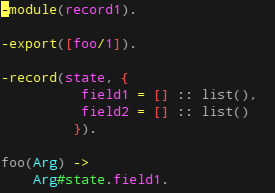
\includegraphics[scale=0.45]{../figures/test1}
&
  	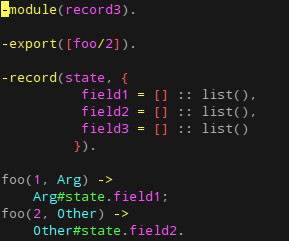
\includegraphics[scale=0.45]{../figures/test2}
\end{tabular}
\end{center}

\end{frame}

\begin{frame}
\frametitle{Non trivial cases}

\begin{itemize}
	\item Escape cases
	\begin{itemize}
		\item Replicate
		\item Return
		\item Call
	\end{itemize}
\end{itemize}

\begin{center}
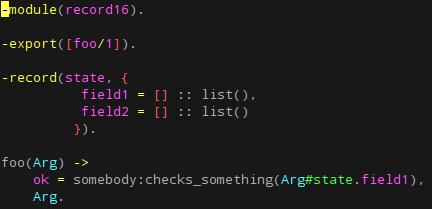
\includegraphics[scale=0.45]{../figures/test16}
\end{center}
\end{frame}

\begin{frame}
\frametitle{Extending to cover the whole language}

\begin{columns}
\begin{column}[l]{3.5cm}

	\begin{block}{}
		\begin{itemize}
			\item \scriptsize{comparisons}
			\item \scriptsize{switches}
			\item \scriptsize{guards}
		\end{itemize}
	\end{block}

	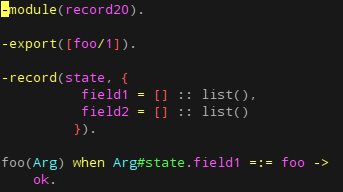
\includegraphics[scale=0.4]{../figures/test20}

\end{column}

\begin{column}[r]{4.5cm}
\begin{tabular}{ c }
  	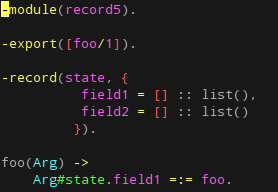
\includegraphics[scale=0.4]{../figures/test5}
\\
	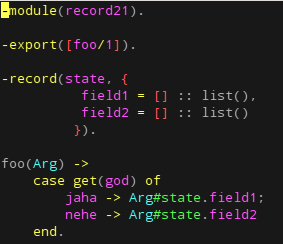
\includegraphics[scale=0.4]{../figures/test21}
\end{tabular}
\end{column}
\end{columns}

\end{frame}

\begin{frame}
\frametitle{Simulating real bugs}

\begin{center}
\begin{tabular}{ c c }
  	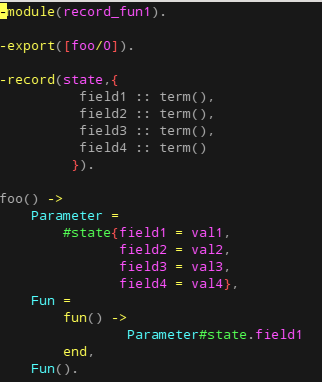
\includegraphics[scale=0.4]{../figures/rec_fun1}
&
	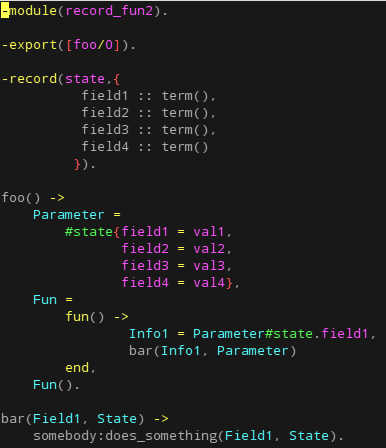
\includegraphics[scale=0.4]{../figures/rec_fun2}
\end{tabular}
\end{center}
\end{frame}

\section{Evaluation Methodology}
\frametitle{Evaluation Methodology}

\begin{frame}

\begin{itemize}
	\item Micro Benchmarks
	\begin{itemize}
		\item Over 30 simple tests
		\item Testing false positives
		\item Testing false negatives
	\end{itemize}
        \pause
	\item Detecting real problems:
	  \begin{itemize}
          \item \textbf{stdlib}:
            \begin{itemize}
            \item 45 warnings
            \item Case study: digraph
            \end{itemize}
          \item \textbf{kernel}:
            \begin{itemize}
            \item 18 warnings
            \end{itemize}
            \pause
          \item \textbf{mnesia}:
            \begin{itemize}
            \item 38 warnings
            \item Case study: mnesia\_controller
            \end{itemize}
            \pause
          \item \textbf{dialyzer}:
            \begin{itemize}
            \item 14 warnings
            \item Case study: dialyzer\_dataflow
            \end{itemize}
	\end{itemize}
\end{itemize}

\end{frame}


\section{Future Work}
\frametitle{Future Work}

\begin{frame}

\end{frame}


\section*{Questions}
\begin{frame}
\begin{block}{}
\begin{center}
\Huge Questions?
\end{center}
\end{block}
\end{frame}

\end{document}
